\documentclass[]{article}
\usepackage{lmodern}
\usepackage{amssymb,amsmath}
\usepackage{ifxetex,ifluatex}
\usepackage{fixltx2e} % provides \textsubscript
\ifnum 0\ifxetex 1\fi\ifluatex 1\fi=0 % if pdftex
  \usepackage[T1]{fontenc}
  \usepackage[utf8]{inputenc}
\else % if luatex or xelatex
  \ifxetex
    \usepackage{mathspec}
  \else
    \usepackage{fontspec}
  \fi
  \defaultfontfeatures{Ligatures=TeX,Scale=MatchLowercase}
\fi
% use upquote if available, for straight quotes in verbatim environments
\IfFileExists{upquote.sty}{\usepackage{upquote}}{}
% use microtype if available
\IfFileExists{microtype.sty}{%
\usepackage{microtype}
\UseMicrotypeSet[protrusion]{basicmath} % disable protrusion for tt fonts
}{}
\usepackage[margin=1in]{geometry}
\usepackage{hyperref}
\hypersetup{unicode=true,
            pdftitle={Risk Benefit Analysis for Toast-USB Launch},
            pdfauthor={Alli McCarty, Nick Mobley, Nijia Ke},
            pdfborder={0 0 0},
            breaklinks=true}
\urlstyle{same}  % don't use monospace font for urls
\usepackage{graphicx}
% grffile has become a legacy package: https://ctan.org/pkg/grffile
\IfFileExists{grffile.sty}{%
\usepackage{grffile}
}{}
\makeatletter
\def\maxwidth{\ifdim\Gin@nat@width>\linewidth\linewidth\else\Gin@nat@width\fi}
\def\maxheight{\ifdim\Gin@nat@height>\textheight\textheight\else\Gin@nat@height\fi}
\makeatother
% Scale images if necessary, so that they will not overflow the page
% margins by default, and it is still possible to overwrite the defaults
% using explicit options in \includegraphics[width, height, ...]{}
\setkeys{Gin}{width=\maxwidth,height=\maxheight,keepaspectratio}
\IfFileExists{parskip.sty}{%
\usepackage{parskip}
}{% else
\setlength{\parindent}{0pt}
\setlength{\parskip}{6pt plus 2pt minus 1pt}
}
\setlength{\emergencystretch}{3em}  % prevent overfull lines
\providecommand{\tightlist}{%
  \setlength{\itemsep}{0pt}\setlength{\parskip}{0pt}}
\setcounter{secnumdepth}{0}
% Redefines (sub)paragraphs to behave more like sections
\ifx\paragraph\undefined\else
\let\oldparagraph\paragraph
\renewcommand{\paragraph}[1]{\oldparagraph{#1}\mbox{}}
\fi
\ifx\subparagraph\undefined\else
\let\oldsubparagraph\subparagraph
\renewcommand{\subparagraph}[1]{\oldsubparagraph{#1}\mbox{}}
\fi

%%% Use protect on footnotes to avoid problems with footnotes in titles
\let\rmarkdownfootnote\footnote%
\def\footnote{\protect\rmarkdownfootnote}

%%% Change title format to be more compact
\usepackage{titling}

% Create subtitle command for use in maketitle
\providecommand{\subtitle}[1]{
  \posttitle{
    \begin{center}\large#1\end{center}
    }
}

\setlength{\droptitle}{-2em}

  \title{Risk Benefit Analysis for Toast-USB Launch}
    \pretitle{\vspace{\droptitle}\centering\huge}
  \posttitle{\par}
    \author{Alli McCarty, Nick Mobley, Nijia Ke}
    \preauthor{\centering\large\emph}
  \postauthor{\par}
      \predate{\centering\large\emph}
  \postdate{\par}
    \date{3/18/2021}

\usepackage{booktabs}
\usepackage{longtable}
\usepackage{array}
\usepackage{multirow}
\usepackage{wrapfig}
\usepackage{float}
\usepackage{colortbl}
\usepackage{pdflscape}
\usepackage{tabu}
\usepackage{threeparttable}
\usepackage{threeparttablex}
\usepackage[normalem]{ulem}
\usepackage{makecell}

\begin{document}
\maketitle

\hypertarget{abstract}{%
\subsection{Abstract:}\label{abstract}}

The popularity of toast as an American breakfast food as well as recent
trends in technology have created a potential marketspace for the
Toast-USB, which allows individuals to curate gourmet toast straight
from their computer. We performed a risk-benefit analysis on two samples
obtained from Toast Co.'s Department of Experiments (DOE) to investigate
the potential favorable response rate for the product as well as
potential target demographic groups for the marketing campaign. A series
of logistic models were built to investigate the potential success of
this product. We found that the best logistic model included demographic
variables representing loan, age, default, and education as demographic
indicators of interest. However, the favorable response rate for the
product was 12.14\%, which was roughly half of the necessary response
rate required for launch of the product. Thus, based on this
risk-benefit analysis, we do not recommend that Toast-Co move forward
with this campaign. However, we do have some actionable next-step
suggestions for Toast-Co to implement to continue their exploration in
this exciting market space.

\hypertarget{introduction}{%
\subsection{Introduction:}\label{introduction}}

Toast has been a staple in the American breakfast for many decades.
Avocado and hummus toast has also been the center of Millennial and
Gen-Z dietary trends, creating a surge in the popularity of gourmet
toast. The sustained popularity of toast as a breakfast food coupled
with a recent drive in demand for gourmet toast created a potentially
high-potential market space to combine toast with technology. Our
client, Toast Co., is aiming to capitalize on a first-mover advantage
and explore this new potential market space. Thus, Toast Co., has
created the Toast-USB which enables individuals to curate gourmet,
artisanal toast right from their computer.

Our aim is to assist Toast Co.~to make informed, data-driven decisions
regarding the launch of Toast-USB. Toast Co.~conducted a first round
market analysis from five metropolitan areas (including Toronto, ON; New
York City, NY, Philadelphia, PA; Dallas, TX, and San Francisco, CA).
Preliminary results were so promising that our firm's DOE has conducted
another larger-scale study to determine the likelihood of success of
Toast-USB. During the course of this investigation, we will synthesize
the key findings from the first and second study. This includes
significant data processing to both reconcile the data of the first and
second study, as well as to process demographic data such that it can be
used in model analysis. Further exploratory analysis will be performed
to investigate key demographic groups that are significant predictors of
a favorable response rate. To perform a risk-benefit analysis on
continuation of the campaign, we will build a series of logistic models
using demographic predictors of interest, and use cross validation based
on maximizing the likelihood ratio to select the model. The model
selection should provide insight on which demographic groups should be
targeted by the marketing campaign, should Toast Co.~move forward with
the launch. Next, we will predict the favorable response rate based on
the selected model, and give a binary(Y/N) recommendation on launch of
the product. Finally, we will determing an MSRP for the product using a
simulation of the logistic model.

\hypertarget{the-data}{%
\section{The Data}\label{the-data}}

The original dataset obtained from Toast Co.'s market analysis contained
421 observations of 8 variables, including 6 categorical variables and 2
numeric variables. The data used for supplementary analysis was provided
by our firm's DOE where additional respondents were sampled from the
same 5 major metropolitan areas to supplement the initial campaign,
which gathered information on 45,211 observations for 16 different
variables, including 9 categorical variables and 7 numeric variables.
Variables relating to the demographic information of the respondents
were all self reported, while variables pertaining to duration of
contact and number of contacts were recorded by campaign administers.
Description of all variables can be found in the data dictionary of the
appendix.

\hypertarget{examining-missing-data}{%
\subsubsection{Examining Missing Data}\label{examining-missing-data}}

From the given data there are 45,211 observations. However there are
17,216 (38.10\%) observations that contain one or more missing values.
Certain categorical variables had missing values with no clear pattern
of missingness. These variables included job, education, contact,
previous days from contact, personal loan status, default status,
marital status, and education. With these variables we decided to add
another category termed ``Unknown'' to represent observations where the
respondents elected to either not respond or were unable to provide
adequate information. However we still needed to address observations
that had missing values in the continuous variables.

We first wanted to understand if the continuous variables were missing
in any distinct pattern. From Figure 1, it appears that the data is
missing at random. In Figure 1, the red cells represent variables that
are missing for a specific pattern, while the numbers on the left
represent how many instances that pattern appeared in the data set. The
number at the bottom of the graphic represents the total number of times
the variable of the column was missing. The graphic suggests that we
only observed 3 rows in which the pattern had 3 missing variables at
once. These three patterns only appeared 13 times in our data set. The
infrequency of these patterns signify that these patterns did occur
randomly. Furthermore, there were 6 distinct patterns that were missing
2 or more variables with a total of 439 occurrences. Since all the
patterns of missing data occurred with a low frequency, it is assumed
that all of our missing values are missing at random. This reinforces
that the quality of sampling and surveying conducted by the DOE, as well
as gives us the freedom to either delete or impute the missing values
without the worry of skewing the data inappropriately.

\begin{figure}
\centering
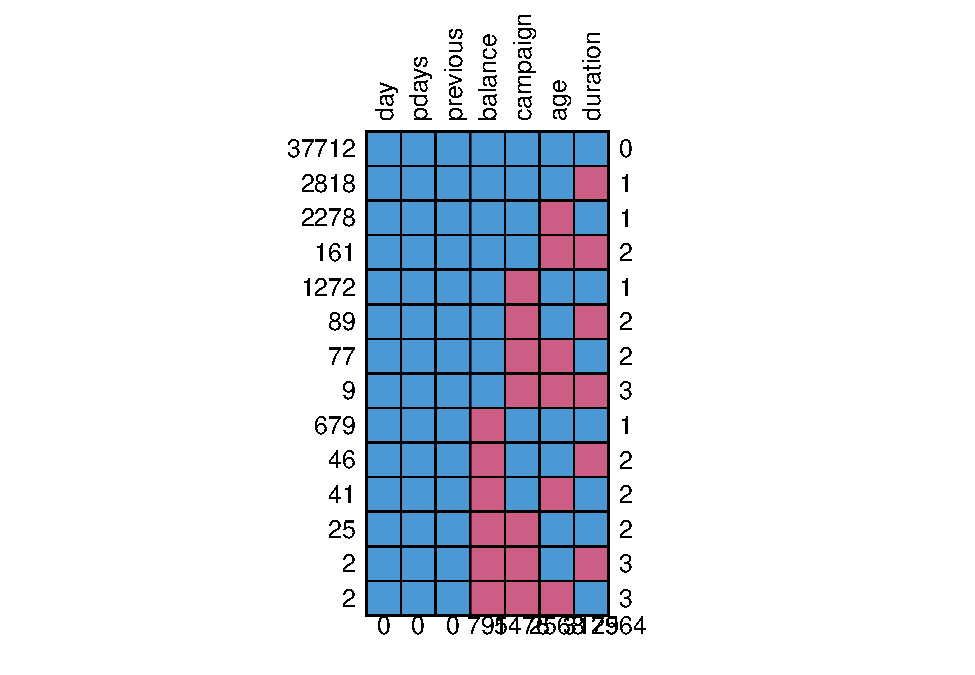
\includegraphics{Compiled-Technical-Report_files/figure-latex/unnamed-chunk-1-1.pdf}
\caption{Missingness pattern of continuous variables in the second
study}
\end{figure}

\begin{verbatim}
##       day pdays previous balance campaign  age duration     
## 37712   1     1        1       1        1    1        1    0
## 2818    1     1        1       1        1    1        0    1
## 2278    1     1        1       1        1    0        1    1
## 161     1     1        1       1        1    0        0    2
## 1272    1     1        1       1        0    1        1    1
## 89      1     1        1       1        0    1        0    2
## 77      1     1        1       1        0    0        1    2
## 9       1     1        1       1        0    0        0    3
## 679     1     1        1       0        1    1        1    1
## 46      1     1        1       0        1    1        0    2
## 41      1     1        1       0        1    0        1    2
## 25      1     1        1       0        0    1        1    2
## 2       1     1        1       0        0    1        0    3
## 2       1     1        1       0        0    0        1    3
##         0     0        0     795     1476 2568     3125 7964
\end{verbatim}

\hypertarget{imputing-continous-variables}{%
\subsubsection{Imputing Continous
Variables}\label{imputing-continous-variables}}

After determining that the four variables containing missing values
(balance, campaign, age, and duration) were all missing at random, we
decided to address this issue by performing a single imputation of the
median to replace the missing values. We conducted an imputation, as
opposed to deleting all observations with missing data in an attempt to
preserve the information of the other 15 variables in these 7,964
observations.

We determined that the median, as opposed to the mean, was the
appropriate measurement to impute the values since all the variables of
interest except age where all right-skewed. Because the variables were
skewed, replacing the missing values with the mean would have
drastically shifted the imputed data sets distributions farther to the
right than expected. This median is not susceptible to skewness meaning
the new imputed distributions will be representative of the original
data set.

\hypertarget{specific-aims-1-to-compare-the-demographic-features-of-the-sample-from-the-first-study-to-that-of-the-second-study-qualitatively-and-quantitatively.}{%
\subsection{Specific Aims 1: To compare the demographic features of the
sample from the first study to that of the second study qualitatively
and
quantitatively.}\label{specific-aims-1-to-compare-the-demographic-features-of-the-sample-from-the-first-study-to-that-of-the-second-study-qualitatively-and-quantitatively.}}

\hypertarget{graphic-comparison-for-the-first-and-second-sample}{%
\subsubsection{Graphic Comparison for the First and Second
Sample}\label{graphic-comparison-for-the-first-and-second-sample}}

We first compare the demographic features common in both studies,
including two numeric variables age and non-mortgage loan balance, as
well as five categorical variables job, education, marital status,
mortgage and primary phone.

To determine whether the decision to purchase the product is
statistically associated with the numeric variable age in the second
study, we generated a boxplot to compare the age distribution of
respondents who are willing to purchase the product against those who
are not. As is shown in Figure 2, people who are willing to purchase the
product have a slightly wider range of age than those who aren't, but
overall, the means of two populations appear to be only slightly
different. However, based on the Welch Two sample t-test, we verified
that the means are significantly different.

\begin{figure}

{\centering 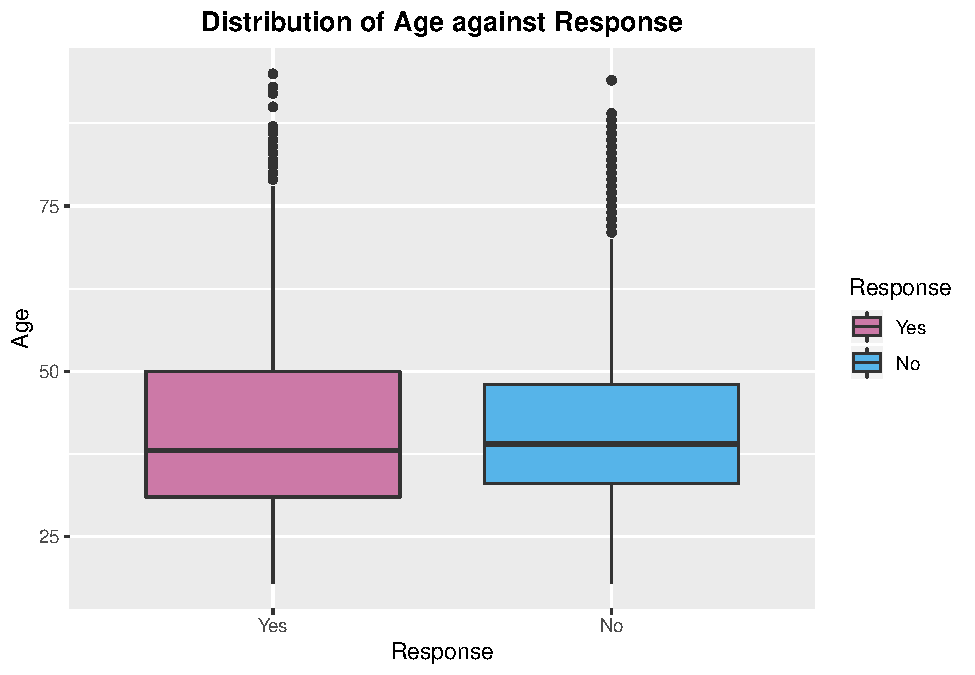
\includegraphics{Compiled-Technical-Report_files/figure-latex/unnamed-chunk-3-1} 

}

\caption{Age distribution of respondents against response in the second study}\label{fig:unnamed-chunk-3}
\end{figure}

To compare the results with the first study, we further obtained the
95\% confidence intervals for the age of people in two populations as
delineated by whether they are willing to purchase the product. We are
95\% confident that respondents who agree to purchase the product are
from 23 to 74 years old, and those who refuse to purchase the product
are from 25 to 60 years old. As provided in the first study, the mean
age of individuals who agree to purchase the product is 25.5, falling
fairly close to the lower bound of the 95\% confidence interval in the
second study, so it's likely that people who are willing to buy the
products from the two studies are not representing the same population.
However, the mean age of respondents who refused to buy the product is
37.5, which is close to the mean age of the counterpart in the second
study (39 years old). Overall, we believe that based on age, samples in
the two studies are unlikely from the same population.

Next, to determine whether the choice to purchase the product is
statistically associated with another numeric variable non-mortgage loan
balance in the second study, we generated a density plot to compare the
age distribution of respondents who are willing to purchase the product
against those who are not, as is shown in Figure 3. The graph indicates
that both distributions are right skewed, and they overlap to a great
proportion with the distribution of respondents who refuse to buy the
product being slightly less right skewed. It can be inferred that
respondents who refused to buy the product might have a lightly lower
balance on average, and as verified by Welch Two sample t-test, the true
means of two populations are significantly different.

\begin{figure}

{\centering 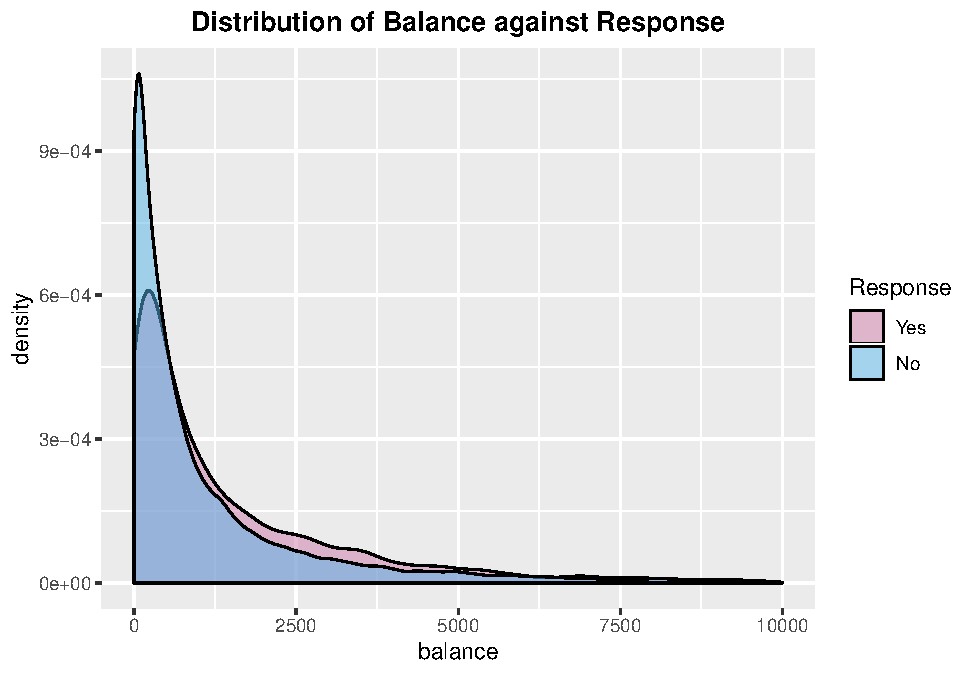
\includegraphics{Compiled-Technical-Report_files/figure-latex/unnamed-chunk-4-1} 

}

\caption{Distribution of non-mortgage loan balance against response in the second study}\label{fig:unnamed-chunk-4}
\end{figure}

We also obtained the 95\% confidence intervals for the non-mortgage loan
balance of people in two populations as delineated by whether they are
willing to purchase the product. We are 95\% confident that in the
second study, respondents who agree to purchase the product have
non-mortgage loan balance between -157.45 and 10185 dollars, and those
who refuse to purchase the product have non-mortgage loan balance
between -393 and 8266 dollars. Similar to the varible age, the average
non-mortgage loan balance of individuals who refuse to purchase the
product (\$1250) in the first study falls within the 95\% confidence
interval of its counterpart in the second study. However, the average
non-mortgage loan balance of individuals who agree to purchase the
product is 23879 dollars, being way higher than the upper limit of its
counterpart in the second study, the sample in the first study is
unlikely from the same population of the second study.

Next, that, we continued to compare the categorical varible job in both
studies. Figure 4 shows the number of respondents of each type of job in
the second study as delineated by their responses to buy the product,
which is ranked by the order of counts in the refusal group from high to
low. Regardless of the reponse, it appears that most of the respondents
are blue-collar, technician or involved in management, but students and
households only take up a fairly small proportion of the sample.

\begin{figure}

{\centering 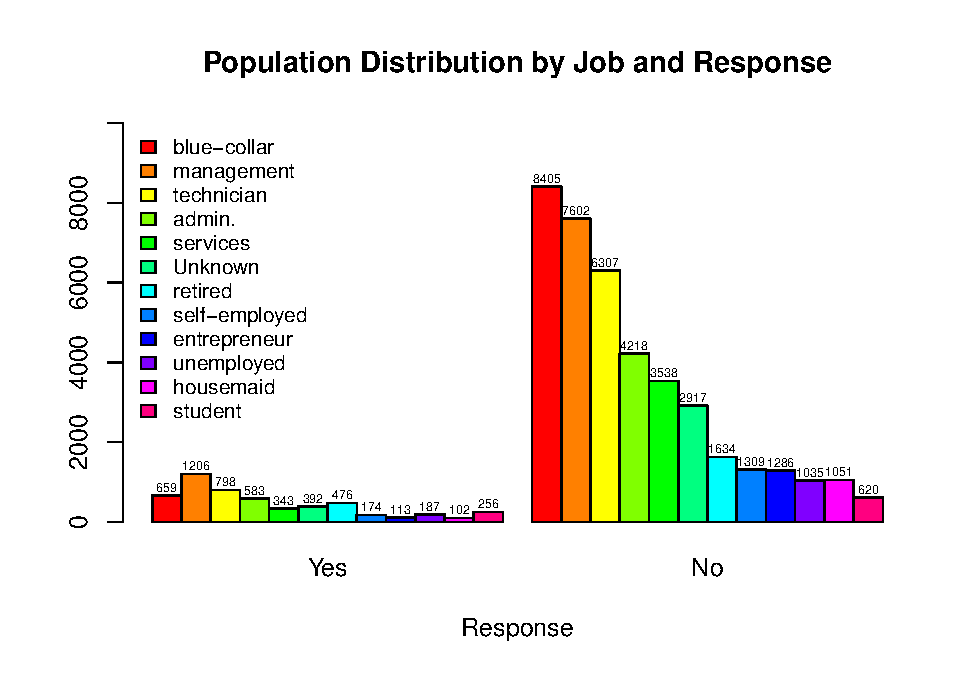
\includegraphics{Compiled-Technical-Report_files/figure-latex/unnamed-chunk-5-1} 

}

\caption{Population distribution of respondents by job and response in the second study}\label{fig:unnamed-chunk-5}
\end{figure}

In order to allow for the comparison of job distributions in the two
studies, we collapsed blue-collar and technician into one category,
counted respondents who are entrepreneurs, administrators or involved in
management as white-collar and combined unemployed and unknown into one
category. Households and students are directly considered as single
levels of the job factor. With all the remaining job types omitted, we
generated barplots in Figure 5 to compare the distributions against
response. In stark contrast to what we observed for the second study, in
the first study, the most common job is student, whereas blue collars
are hardly seen. This clearly indicates that according to job type, the
two studies are not based on the same population.

\begin{figure}

{\centering \includegraphics{Compiled-Technical-Report_files/figure-latex/unnamed-chunk-7-1} 

}

\caption{Population distribution of respondents by job and response in both studies}\label{fig:unnamed-chunk-7}
\end{figure}

\begin{figure}

{\centering \includegraphics{Compiled-Technical-Report_files/figure-latex/unnamed-chunk-8-1} 

}

\caption{Population distribution of respondents by education and response in both studies}\label{fig:unnamed-chunk-8}
\end{figure}

We also compared the distribution of respondents with different
education backgrounds as delineated by their response to purchase the
product, as is shown in Figure 5. The tertiary education in the second
study can be regarded as the the same as the college and more level in
the first study, so the relevant bars were all highlighted in red. From
the figures, we can see that although there're similar numbers of
respondents who agree or refuse to buy the product in the first study,
in the second study there're apparently more respondents who refuse to
buy the products than agree. The majority of the respondents involved in
the first study has education level of college or higher, whereas in the
second study , there's less respondents with college education than
respondents with secondary education. It seems that based on education
levels, these two studies are not from the same population.

\begin{figure}

{\centering \includegraphics{Compiled-Technical-Report_files/figure-latex/unnamed-chunk-9-1} 

}

\caption{Population distribution of respondents by marital status and response in both studies}\label{fig:unnamed-chunk-9}
\end{figure}

Similarly, We also compared the distribution of respondents with
different marital status against their response to purchase the product,
as is shown in Figure 6. In the first study, there're significantly
lower numbers of married respondents than not married respondents,
whereas there're about equal total numbers of married respondents as
those not married. Therefore, these two samples are unlikely from the
same population. Interestingly, if we focus on the distribution of
married respondents in both studies, we can see that in both study,
married respondents are unlikely to purchase the product.

\begin{figure}

{\centering \includegraphics{Compiled-Technical-Report_files/figure-latex/unnamed-chunk-10-1} 

}

\caption{Population distribution of respondents by mortgage and response in both studies}\label{fig:unnamed-chunk-10}
\end{figure}

Furthermore, we compared the distribution of respondents with or without
mortgage against their response to purchase the product, as is shown in
Figure 7. Similar to what we observed in Figure 6, in the first study,
the majority of the respondents are without mortgage, whereas in the
second study there are about comparable number of respondents who have
mortgage or not. This could serve as edividence to show that the second
study was well designed to randomize the sample. To our notice, in both
studies, people with mortgage are less likely to purchase the product as
compared to those with no mortgage. This could be explained as if people
with mortgage are more prudent with how they should spend money.
However, we see conflicting trends of response in the two studies among
the group with no mortgage, which could result from the difference in
sampling.

\begin{figure}

{\centering \includegraphics{Compiled-Technical-Report_files/figure-latex/unnamed-chunk-11-1} 

}

\caption{Population distribution of respondents by primary phone and response in both studies}\label{fig:unnamed-chunk-11}
\end{figure}

With regard to the distribution of respondents use cell phone or not as
their primary phone against their response to purchase the product
(shown in Figure 8), it appears that less than half ot the respondents
use cell phone as their primary phone in the first study, whereas more
than half of the respondents use cell phone as their primary phone in
the second study. The second study may be representing the usual cases,
as nowadays people tend to use cell phone more often than before.
Interestingly, although respondents who use cell phones as their primary
phone tend to agree to buy the product in the first study, this trend is
reversed in the second study, with the majority of the respondents
refused to buy the product. Apparently, these two samples are not from
the same population.

\begin{figure}

{\centering \includegraphics{Compiled-Technical-Report_files/figure-latex/unnamed-chunk-12-1} 

}

\caption{Comparison of the population distribution by delinquency and response in the first study against the population distribution by credit in default and response in the second study}\label{fig:unnamed-chunk-12}
\end{figure}

It's possible that people in delinquency for more than 60 days also have
credit in default, so we compared the delinquency variable in study one
with the credit in default varible in study 2, as is shown in Figure 9.
To our notice, the great majority of the respondents in the second study
are do not have credit in default, whereas in the first study
respondents that have less than 60 days of delinquency account for only
slightly more than half of the whole sample. Interestingly, in the first
studies, respondents that has less than 60 days of delinquency are less
likely to buy the products, and a similar trend is observed in the
second study, where the majority of repondents with no credit in default
refuse to buy the product.

\begin{figure}

{\centering \includegraphics{Compiled-Technical-Report_files/figure-latex/unnamed-chunk-13-1} 

}

\caption{Population distribution of respondents by gender against response or by race against response in the first study}\label{fig:unnamed-chunk-13}
\end{figure}

Now that the variables common in both studies have been scrutinized, we
continued to examine the pattern of distributions with variables only
described in the first study, including gender and race. Figure 10
displays the side-by-side distribution of respondents of different
gender or race against response. It appears that male and white people
both take up the majority of the respondents, which could potentially
lead to biased response rates.

\begin{figure}

{\centering \includegraphics{Compiled-Technical-Report_files/figure-latex/unnamed-chunk-14-1} 

}

\caption{Population distribution of respondents by personal loan and response in the second study}\label{fig:unnamed-chunk-14}
\end{figure}

In the second study, whether or not a respondent has personal loan is
the only variable reflecing demographic features that haven't been
looked into. Consistent with what we observed for the credit in default
variable, the majority of the respondents are with no personal loan.
Interestingly, regardless of having personal loan or not, they both tend
to not buy the product, with similar probabilities.

\newpage

\hypertarget{likelihood-ratio-tests}{%
\subsubsection{Likelihood ratio tests}\label{likelihood-ratio-tests}}

Next, we conducted likelihood ratio tests to examine whether response to
purchase the product is dependent on each categorical variable
reflecting demographic features. For the first study, likelihood ratio
test statistics, degrees of freedom and p-values of the tests on the
eight variables (job, education, marital status, mortgage, primary
phone, delinquency, gender and race) has been shown in Table 1, with all
of the p-values being less than 0.05, indicating that there is
significant evidence that response to buy the product are associated
with each of these eight variables.

\begin{table}
    \centering
    \begin{tabular}{ |c | c | c | c | c |}
    \hline
        Variable & Levels & G2 & df & P-value \\ \hline
        Job & White Collar, Blue Collar, Student, House, Unemployed or Unknown & 321.67 & 4 & < 0.001 \\ \hline
        Education & College and more, Lower than college & 31.92 & 1 & < 0.001 \\ \hline
        Marital & Married, Not married & 71.97 & 1 & < 0.001 \\ \hline
        Mortgage & Mortgage, No Mortgage & 19.49 & 1 & <0.001 \\ \hline
        Primary Phone & Cellular, Other & 68.66 & 1 & <0.001 \\ \hline
        Delinquency & More than 60 days, 60 or less days & 113.33 & 1 & <0.001 \\ \hline
        Gender & Male, Female & 6.81 & 1 & 0.009 \\ \hline
        Race & White, Not White & 4.08 & 1 & 0.043 \\ \hline
    \end{tabular}
    \caption{Table 1}
\end{table}

(insert Table 1)

Similarly, Table 2 reflects the likelihood ratio tests of whether
response to purchase the product is dependent on each of the demographic
categorical variable in the second study, including job, education,
marital status, mortgage, primary phone, credit in default and personal
loan. The categories used are based on the original levels of factors in
the second study. the Similar to what we observed in Table 1, all of the
p-values are less than 0.05, suggesting that there're significant
evidence that response to buy the product are dependent on each of these
seven variables.

(insert table 2)

Since for response is statistically associated with each of the five
categorical variables common in both studies, we further conducted five
more likelihood ratio tests to examine whether the samples in the two
studies are from the same population. Assuming that they are two samples
from the same population, then the proportion of each level of the
interaction terms of response and any of the five categorical variables
should be the same for both studies. To allow for the comparisons, the
categories used are based on the original levels of factors in the first
study. The test statistics are shown in Table 3. As expected, the
p-values are all less than 0.05, which confirms that the components of
respondents in the first study are significantly different from that in
the well randomized second study.

(insert table 3)

\hypertarget{exploratory-data-analysis-for-modeling-process}{%
\subsubsection{Exploratory Data Analysis for Modeling
Process}\label{exploratory-data-analysis-for-modeling-process}}

For this study we were interested in creating a logistic model that was
able to capture how the likelihood that a person would buy the product
based off of their demographic information. This is in effort to create
a generalized model that can be used to predict the success of the
Toast-USB.

First, we want to explore the relationship between the demographic
variables in the sample, and particularly explore how demographic
information affects willingness to purchase Toast-USB. In this case, we
can define willingness to purchase the Toast-USB as both the binary
(Y/N) favorable response and the price a person said they would be
willing to pay for the product. Figure X shows the relationship between
age and willingness to purchase. There is a moderate relationship
between age and price, and the figure suggests that individuals on the
older end of the spectrum may actually have more a more favorable
response to the product. This is somewhat contridictory to our
expectation, given that Millennial and Gen-Z's dual love for technology
and gourmet toast served as a compelling reason to enter this market
space with the launch of the Toast-USB. This paradoxical relationship
could be due to the fact that younger people are more likely to eat-out
rather than at home, and therefore are less likely to purchase kitchen
appliances. Additionally, young people establishing their first
household may have access to less capital to purchase appliances,
resulting in a decreased willingness to purchase among this demographic
group. The figure also demostrated that people had a favorable response
to the product were also, on average, willing to pay more for the
product.

Next, in Figure X we explored the relationship between logged-balance
and willingness to purchase. Balance representes the amount of
non-morgatage credit currently owed by an individual. If a person has a
large balance, it could negatively impact their willingness to purchase
the Toast-USB simply because they do not have access to capital. The
metric representing balance had both negative values and a strong
right-skew. We performed a linear shift by the largest negative-value
balance and a log-transformation to alleviate the skew of the date. The
equation below represents the mathematical formula used to transform the
balance variable:

\(Transformed Balance = log(Balance + min(Balance))\)

Figure X represents the association between logged balance and
willingness to purchase Toast-USB. The figure does not demonstrate that
there is a significant association between balance and willingness to
purchase. Similarly to the relationship demonstrated for age, the figure
also suggests that people with a favorable respone were, on average,
willing to pay more for Toast-USB.

\includegraphics{Compiled-Technical-Report_files/figure-latex/unnamed-chunk-15-1.pdf}

\includegraphics{Compiled-Technical-Report_files/figure-latex/unnamed-chunk-16-1.pdf}

\includegraphics{Compiled-Technical-Report_files/figure-latex/unnamed-chunk-17-1.pdf}

Figure X demostrated the association between continuous demographic
predictors and willingness to purchase the product. None of the
variables have a particularly strong association with willingness to
purchase, and there are no obvious instances of collinearity between the
continuous demographic predictors. However, the plots of the continuous
predictors do suggest that price is a significant seperator. As
demonstrated in previous exploratory analysis, individuals who had a
favorable response to the product were also willing to pay more for it
than people who did not have an initial favorable response.

\includegraphics{Compiled-Technical-Report_files/figure-latex/unnamed-chunk-18-1.pdf}

Figure X shows the association between categorical demographic
predictors and their willingness to purchase the Toast-USB. Variables
representing education, default, and loan have a moderate relationship
with willingness to purchase. Individuals with secondary and tertiary
education have a higher favorable response rate, which could be dually
attributable to access to more capital and cultural trends surrounding
gourmet toast that are popular within this group. Additionally, there is
a moderate association between willingness to purchase, loan, and
default. We believe that these associations could be related, as
individuals with secondary and tertiary education (specifically,
individuals attended college) are more likely to have a non-morgatage
loan due to the exorbanant cost of education in the United States. The
association of these three variables should be considered in the
structure of the logistic model.

\includegraphics{Compiled-Technical-Report_files/figure-latex/unnamed-chunk-19-1.pdf}

The original dataset obtained by the DOE had 12 factors representing the
job classification for individuals in the sample. The job variable was
recoded to represent more broad categories more closely related to
profession-type. Factor levels in the recoded dataset for
profession-type include classifications of student, unknown employment,
administration, white-collar, and blue-collar. Figure X represents the
distribution of favorable response for each of the profession types.
There is no significant association between favorable response and
profession type in this sample.

\includegraphics{Compiled-Technical-Report_files/figure-latex/unnamed-chunk-20-1.pdf}

After exploratory analysis, we believe that default, education, loan,
and age are demographic variables of interest that could be utilized in
the logistic model. For the statistical analysis portion, we aim to
build a logistic model that uses relevant demographic variables to
predict a favorable response to the Toast-USB and indicate if
Toast-Co.~should move forward with the launch of the produce.

\hypertarget{model-process}{%
\subsection{Model Process}\label{model-process}}

We identified that default, education, loan, and age were potentially
significant indicators of willingness to purchase in the exploratory
analysis. Our aim for the analysis was to 1) predict the success of the
Toast-USB and 2) indicate which demographic groups should be targeted in
the marketing campaign. To investigate these endpoints, we generated a
function that build a multivariate logistic models representing every
combination of the four aforementioned variables. Interaction terms were
not included, as none of these variables demonstrated significant
collinearity. To do so, we partitioned the data into a test and a train
set, both of which represented half of the original dataset
(non-overlapping). Using the train-set, we generated 15 potential
logistic models representing combinations of these four predictors.
Next, we generated a function to cross-validate the models using the
test-set to select the model with the maximal likelihood ratio.

\begin{verbatim}
## y ~education+loan+age 
##                    14
\end{verbatim}

\begin{verbatim}
## 
## Call:
## glm(formula = bestFormula, family = binomial, data = training)
## 
## Deviance Residuals: 
##     Min       1Q   Median       3Q      Max  
## -0.7254  -0.5346  -0.4811  -0.4041   2.5545  
## 
## Coefficients:
##                     Estimate Std. Error z value Pr(>|z|)    
## (Intercept)        -2.341301   0.121384 -19.288  < 2e-16 ***
## educationprimary   -0.450160   0.102507  -4.391 1.13e-05 ***
## educationsecondary -0.114468   0.086869  -1.318  0.18760    
## educationtertiary   0.230625   0.088570   2.604  0.00922 ** 
## loanUnkown         -0.259650   0.226084  -1.148  0.25078    
## loanyes            -0.708115   0.072746  -9.734  < 2e-16 ***
## age                 0.010222   0.002032   5.031 4.87e-07 ***
## ---
## Signif. codes:  0 '***' 0.001 '**' 0.01 '*' 0.05 '.' 0.1 ' ' 1
## 
## (Dispersion parameter for binomial family taken to be 1)
## 
##     Null deviance: 16057  on 22604  degrees of freedom
## Residual deviance: 15817  on 22598  degrees of freedom
## AIC: 15831
## 
## Number of Fisher Scoring iterations: 5
\end{verbatim}

Of the 15 logistic models that were generated using loan, age, default,
and education, we found that the multivariate logistic model regressing
age, loan, and education on response to Toast-USB had the maximum
likelihood ratio. The model summary also indicated that secondary,
tertiary and unknown education, age, a having a loan were significant
predictors in the model. Thus, we believe that education, loan status,
and age will be demographic variables of interest to Toast-Co for
strategizing their marketing campaign. Next,we used our selected
logistic model to simulate a response rate using the testing set.

\begin{verbatim}
## [1] 0.1141783
\end{verbatim}

The favorable response rate for for the product was 12.14\%, which is
approximately half of the necessary response rate that
Toast-Co.~indicated would be necessary for the launch of the product.
Based on this analysis, we do not recommend that Toast Co.~move forward
with this version to Toast-USB.

\hypertarget{sa3-application-of-model-to-determine-msrp}{%
\subsection{SA3 Application of Model to Determine
MSRP}\label{sa3-application-of-model-to-determine-msrp}}

From our previous section we discovered that the logistic model
containing loan,education,age as our predictor variables performed the
best predictions. Although the favorable response is not near the break
even rate we still continued in determining which MSRP value would be
able to maximize revenue. To generate a range of reasonable prices we
selected the minimum and maximum value of price answered in the survey.
The lowest value responded value was 0 but we will start our search at 1
and the maximum responded price was 168 so we will search for the
optimal value in that range. To find the maximum price we performed the
following simulation: For each potential MSRP Value: Repeat the below
following process 5 times and take the average: For each observation in
our training set: 1. Generate a probability they would purchase the
product using the logistic model 2. Compare that generated probability
with a randomly generated number, if the random number is lower than the
probability then the customer will consider purchasing the item. If not
then we skip to next observation. 3. We compare the MSRP to observed
price the customer said they were willing to pay. If the MSRP is less
than than the price then in our simulation the customer ``purchases''
the product and that sale is added to the total revenue and we continue
to the next observation. We key the total revenue to be associated with
the MSRP value and selected the MSRP value with the highest revenue.

\includegraphics{Compiled-Technical-Report_files/figure-latex/unnamed-chunk-23-1.pdf}

From the results of our simulation we can see that the estimated maximum
MSRP Value would \$46. The simulation was ran on a test set containing
20,000 observations. From this we could estimate that for every 20,000
people that interact with our product we could estimate a revenue of
approximately \$60,000.

\hypertarget{conclusion}{%
\subsection{Conclusion:}\label{conclusion}}


\end{document}
